\documentclass[conference]{IEEEtran}
\usepackage[T1]{fontenc}\usepackage[utf8]{inputenc}
\usepackage{amsmath,graphicx,booktabs,cite}
\begin{document}
\title{ESGenius: AI-Based BRSR Gap Analysis and MSCI-Style ESG Scoring of Sustainability Reports}
\author{\IEEEauthorblockN{Aditya Sinha}\IEEEauthorblockA{Department of Computer Engineering\\Vidyalankar Institute of Technology, Wadala, Mumbai, India} \and \IEEEauthorblockN{Sehaj Alag}\IEEEauthorblockA{Department of Computer Engineering\\Vidyalankar Institute of Technology, Wadala, Mumbai, India} \and \IEEEauthorblockN{Pradnesh Jadhav}\IEEEauthorblockA{Department of Computer Engineering\\Vidyalankar Institute of Technology, Wadala, Mumbai, India} \and \IEEEauthorblockN{Gaurav Deore}\IEEEauthorblockA{Department of Computer Engineering\\Vidyalankar Institute of Technology, Wadala, Mumbai, India}}
\maketitle
\begin{abstract}The largest listed companies in India have to file a Business Responsibility and Sustainability Report (BRSR) that answers 140 questions set by the Securities and Exchange Board of India (SEBI). Checking a report against every question by hand is slow, and afterwards it is still hard to say how well the company has disclosed. We built ESGenius to help with both problems. A user uploads a sustainability report as a PDF. The system finds the pages that answer each of the 140 questions, then asks a large language model, Google Gemini, through the Gemini API, whether the question is covered, partly covered, not covered or needs a human look. From these answers it works out an MSCI-style ESG score with the structure MSCI publishes: key issue scores, a weighted average, an adjustment against other companies in the same industry, and a rating from AAA to CCC. A reviewer can mark a question as not applicable, for example the water questions of a company that uses no process water, so that it is not counted against the company. ESGenius also writes a PDF gap report and answers questions about the uploaded document. We tested retrieval on one public 49-page report. The top page was relevant for 85.0\% of the questions and at least partly relevant for 92.1\%, as graded by an AI assistant. In a full run on the same report, 53 of the 140 questions were classified and the other 87 were passed to human review when the daily model quota ran out, which is the intended fail-safe. The score shows how well a company discloses, not how well it performs, and it is not an official MSCI rating.\end{abstract}
\begin{IEEEkeywords}ESG scoring, SEBI BRSR, MSCI ESG Ratings, retrieval-augmented generation, large language model, BM25, compliance gap analysis\end{IEEEkeywords}
\section{Introduction}
Since 2021 the largest listed companies in India have had to publish a Business Responsibility and Sustainability Report with their annual report \cite{b1}. The BRSR format asks 140 numbered questions. Section A holds general disclosures and Section B covers management and process. Section C is split over the nine principles of the National Guidelines on Responsible Business Conduct, and each principle has Essential and Leadership indicators.

Two jobs come out of this. A sustainability team has to check that a draft report answers every question and that the answer is backed by data. Investors and reviewers, on the other hand, want one number or letter that tells them how well the company discloses. Rating providers such as MSCI publish letter ratings from AAA to CCC for this purpose \cite{b2}. In both cases someone has to read a report of many pages that mixes prose with tables.

ESGenius does that reading with the help of a large language model (LLM), but the model is not left alone. We retrieve the evidence ourselves with a rule-based search, give the model only that evidence, and add fixed rules for the cases where the model fails. This paper makes four contributions.

First, a gap analysis pipeline. It extracts the text of a PDF page by page, finds evidence for each of the 140 questions and classifies each question with the Gemini LLM.

Second, an MSCI-style ESG score. It is calculated from the classification results with the same steps MSCI describes: key issue scores, a weighted average, an industry adjustment and an AAA to CCC band.

Third, a reviewer control that marks a question as not applicable. Without it, a company would lose points for leaving out information it does not have.

Fourth, a PDF gap report and a document assistant, both with page citations, inside a web application with sign-in and usage limits.

Section II covers related work and Section III the system. Section IV explains the gap analysis and Section V the scoring. Section VI walks through the application screen by screen. Section VII describes implementation and testing, Section VIII gives the evaluation, and Section IX concludes.

\section{Related Work}
Several projects use LLMs on sustainability reports. ChatReport \cite{b7} lets users ask questions about a report and analyse it with an LLM. ESGReveal \cite{b6} combines retrieval with an LLM to pull structured data out of ESG reports. On reports of companies listed in Hong Kong it reached 76.9\% accuracy for data extraction and 83.7\% for disclosure analysis. ClimateBERT \cite{b10} is a language model trained on climate-related text. These works deal with ESG or climate disclosure in general. We work on one regulatory format, the BRSR, and every result points to a numbered question and a PDF page.

ESG ratings are the second area. MSCI scores a company from 0 to 10 on each key issue that matters for its industry, combines the scores with industry-specific weights, compares the result with industry peers and then assigns a letter from AAA to CCC \cite{b2}, \cite{b3}, \cite{b4}. Berg et al. found that the ratings of different providers for the same company often disagree, mainly because of differences in what is measured, which topics are included and how they are weighted \cite{b5}. That is the reason we publish our weights and formulas in full. Fernandez et al. \cite{b8} use machine learning to explain ESG scores from financial data of US companies. Our score goes the other way: it is calculated from what the company writes in its report.

The third area is retrieval and generation. Retrieval-augmented generation gives an LLM retrieved passages to work from instead of asking it to answer from memory \cite{b9}. Dense retrieval is popular, but the lexical BM25 function \cite{b11} is still a strong baseline. BRSR questions use fixed, domain-specific wording, so a lexical search suits them. It gives the same result every time, costs nothing to run and can be inspected. LLMs can also state things the source does not say \cite{b12}, which is why we wrapped the model in fixed rules (Section IV-D).

\section{System Overview}
ESGenius is a web application with a frontend, a backend and a database. Table I lists the technology behind each part and what it does.

\begin{table}[!t]\centering\caption{Technologies Used and Their Role}
\footnotesize\begin{tabular}{lcc}\toprule
Part & Technology & Role \\ \midrule
Frontend & React 19, TypeScript, TanStack Router and Query, Vite & Upload, progress, results, score \\
Backend & Java 21, Spring Boot 3.4 & REST API, background jobs, scoring \\
Database & PostgreSQL, Flyway migrations & Documents, pages, analyses \\
Sign-in & Supabase Auth (bearer token) & Users, document ownership \\
PDF text & Apache PDFBox & Per-page text, no OCR \\
Retrieval & Own BM25-style lexical retriever & Page-cited evidence \\
LLM & Google Gemini, Gemini API with API key & Classification, assistant \\
\bottomrule\end{tabular}
\end{table}
Fig. 1 shows how a report moves through the system. When a user uploads a PDF, the upload returns at once and a background worker extracts the text and stores it page by page. An analysis also runs in the background, and the browser asks for its progress every two seconds. If the server restarts while a job is running, the job is marked as failed on start-up so that it does not stay pending forever.

Every document belongs to the user who uploaded it. Another user asking for it gets a not-found answer. Uploads are limited to 25 MB, 400 pages and three million characters. Each user also has daily limits on uploads, analyses and assistant questions, which protects the shared model quota.

\begin{figure}[!t]\centering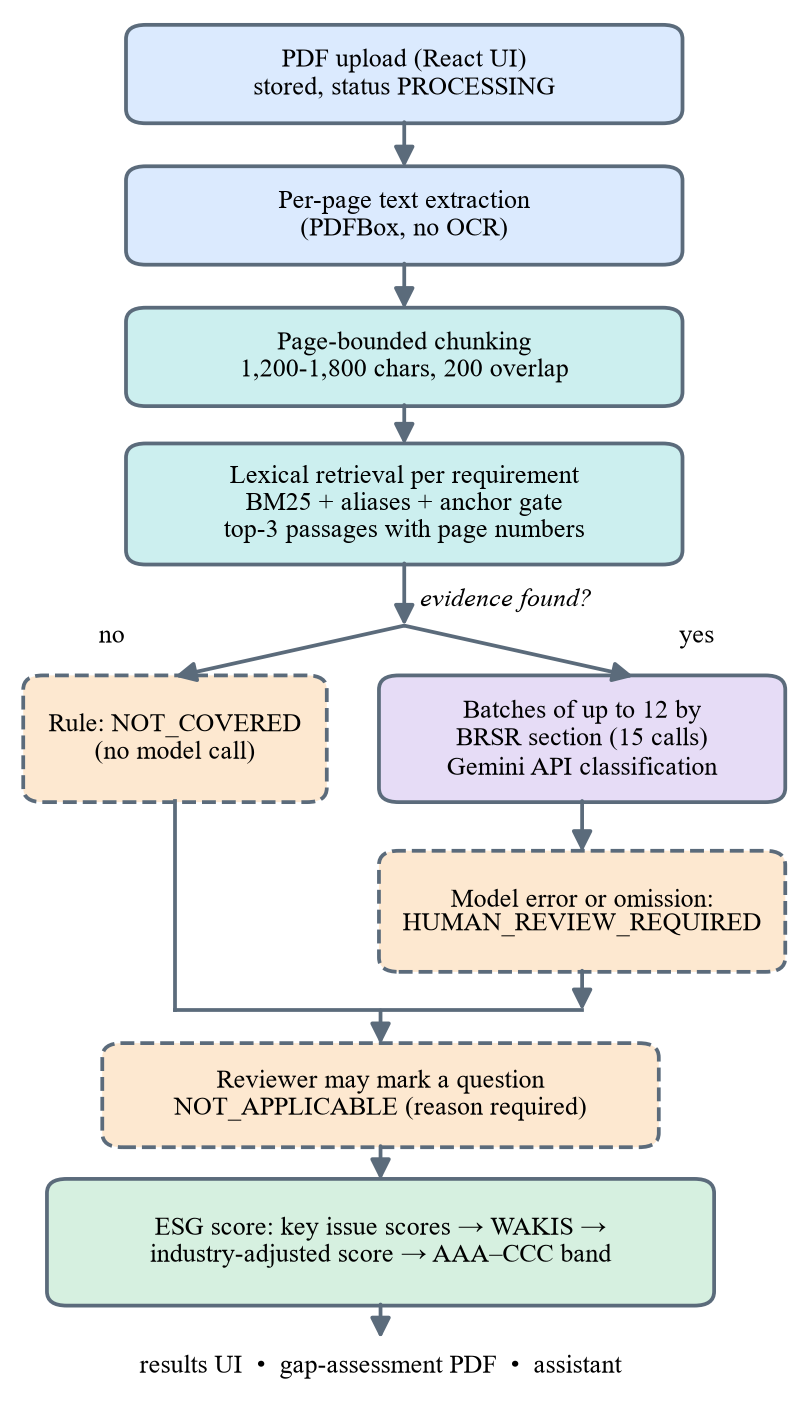
\includegraphics[width=0.95\columnwidth]{fig_v2_pipeline.png}
\caption{ESGenius pipeline from PDF upload to gap analysis, ESG score and report. Dashed boxes are rule-based paths that do not use the model.}\end{figure}
\section{Gap Analysis Method}
\subsection{BRSR Requirement Set}
We stored all 140 questions of the BRSR format as requirements. There are 24 general disclosures in Section A and 12 management and process questions in Section B. Section C adds 104 indicators, 62 Essential and 42 Leadership, spread over Principles 1 to 9. A requirement has a code such as P6-E06, a title, a description, the framework text, its section and its indicator type.

\subsection{Chunking and Evidence Retrieval}
The text of each page is cut into chunks of about 1,200 to 1,800 characters with a 200-character overlap. A chunk never crosses a page boundary, so every passage we retrieve has an exact page number. For each requirement we build a weighted query from its code (weight 3.0), title (6.0) and description (2.5). Stop-words and very common BRSR words are removed, and we add a small list of aliases, for example \textit{bribery} for \textit{corruption}. Every sentence-level passage \textit{p} is scored against each query term \textit{t} with the BM25 term score \cite{b11}:

\begin{equation}s(t,p)=w_t\,\mathrm{idf}(t)\,\frac{\mathrm{tf}_{t,p}(k_1+1)}{\mathrm{tf}_{t,p}+k_1\left(1-b+b\,\frac{|p|}{\bar L}\right)}\end{equation}
Here \textit{w\_t} is the weight of the term, \textit{tf} is how often it occurs in the passage, |\textit{p}| is the passage length, \textit{$\bar{L}$} is the mean chunk length, \textit{k\_1} is 1.2 and \textit{b} is 0.75. The passage score gets extra points for phrase matches such as title phrases and aliases. A passage is only used if it passes an anchor gate, which means it must contain a required phrase or at least two discriminative query terms. We return the three best chunks that score at least 0.15, with their page numbers. If no chunk qualifies, the requirement has no evidence. Before the classification step each passage is widened by a few hundred characters inside its chunk, so that the model also sees a table heading or the sentence before it.

\subsection{Classification with the Gemini API}
Requirements that have evidence are classified by Google Gemini, a large language model \cite{b13}. The backend calls the Gemini API with an API key that is stored in the server configuration. The model answers with one of four statuses (covered, partially covered, not covered, human review required), a confidence value, a short explanation, the gap and a recommendation. The prompt hands the model the requirement title, description and framework text as the full rubric. It tells the model to use only the retrieved evidence, to ignore outside knowledge and not to claim any certification. Because the evidence comes from the uploaded report and is passed to the model together with the requirement, this is retrieval-augmented generation.

Asking one question per call would take 140 calls for one analysis, and the free tier of the API allowed only 20 requests per day. So we group the requirements by BRSR section and split each group evenly into batches of at most \textit{L} = 12 requirements. The prompt lists the rubric and the evidence of every requirement and asks for a JSON array with one entry per requirement code. A full BRSR analysis then needs 15 calls (Table II).

\begin{table}[!t]\centering\caption{Model Calls per Full Analysis (140 Requirements)}
\footnotesize\begin{tabular}{lcc}\toprule
Strategy & Calls & Fits 20/day? \\ \midrule
One call per requirement & 140 & No \\
Section batches, L = 12 & 15 & Yes (5 spare) \\
\bottomrule\end{tabular}
\end{table}
\subsection{Fail-Safe Rules}
The model can never create coverage by itself. A requirement without evidence is marked not covered by a fixed rule and the model is not called. If the model leaves out a requirement or returns a broken entry, that requirement becomes human review required. If a whole call fails, every requirement in that batch becomes human review required. Errors that can go away are retried after the delay the server asks for, and when the daily quota runs out the explanation says so. The status not applicable is out of the model's reach: only a human reviewer can set it. A failure therefore sends work to a person and never produces a false covered.

\subsection{Not-Applicable Questions}
Some questions do not apply to every company. A company that uses no process water has nothing to report about water withdrawal, and an empty answer is correct. Counting it as a gap would be unfair. A reviewer can therefore mark the question as not applicable and has to write a reason. The question then drops out of the score, and the PDF report lists it with that reason. The old status is stored, so the decision can be undone.

\section{MSCI-Style ESG Scoring}
\subsection{The MSCI Structure}
MSCI builds a rating from the bottom up \cite{b2}, \cite{b4}. A company gets a score from 0 to 10 for every key issue that is material for its industry. The key issue scores are combined with industry-specific weights into the Weighted Average Key Issue Score (WAKIS). The WAKIS is then turned into an Industry-Adjusted Score (IAS) between 0 and 10, using the lowest and highest scores in the industry \cite{b3}, and the IAS decides the letter from CCC to AAA. MSCI also gives the governance pillar a weight of at least 33\% \cite{b4}.

\subsection{How ESGenius Applies It}
We keep the same chain of steps, but our input is the BRSR result instead of MSCI's company data. Every classified requirement \textit{r} gets points \textit{p\_r}: 10 if covered, 5 if partially covered and 0 if not covered. Requirements that are not applicable or still need human review are left out. Leadership indicators are voluntary in the BRSR format, so they count with weight 0.5 and all other requirements with weight 1. The score of a key issue \textit{i} is the weighted mean of its requirement points:

\begin{equation}\mathrm{KIS}_i=\frac{\sum_{r\in i}\omega_r\,p_r}{\sum_{r\in i}\omega_r}\end{equation}
We group the BRSR sections into ten key issues and three pillars (Table III). Each of the 140 questions feeds exactly one key issue.

\begin{table}[!t]\centering\caption{Key Issues and the BRSR Sections That Feed Them}
\footnotesize\begin{tabular}{lccc}\toprule
BRSR & Key issue & Pillar & Req. \\ \midrule
A, B & Corporate governance and management systems & Governance & 36 \\
P1 & Business ethics and transparency & Governance & 9 \\
P7 & Responsible policy advocacy & Governance & 3 \\
P2 & Sustainable and safe products and services & Environmental & 9 \\
P6 & Environmental footprint & Environmental & 21 \\
P3 & Employee wellbeing and human capital & Social & 21 \\
P4 & Stakeholder engagement & Social & 5 \\
P5 & Human rights & Social & 15 \\
P8 & Inclusive growth and community development & Social & 10 \\
P9 & Consumer value and responsibility & Social & 11 \\
Total &  &  & 140 \\
\bottomrule\end{tabular}
\end{table}
Every industry has pillar weights \textit{π\_E}, \textit{π\_S} and \textit{π\_G} that add up to 1 (Table IV). MSCI chooses weights from how much an industry contributes to environmental and social problems and how soon the risk shows up \cite{b4}. MSCI's own weight tables are not public, so the values in Table IV are our prototype choices for 11 sectors. They follow the same logic: heavy industry puts most weight on the environment, software and health care on the social pillar, and governance never goes below 33\%. The weight of a pillar is shared equally among its scored key issues, so \textit{W\_i} = \textit{π\_g(i)} / \textit{n\_g(i)}, where \textit{n\_g} is the number of scored key issues in pillar \textit{g}. The WAKIS is then

\begin{equation}\mathrm{WAKIS}=\sum_i W_i\,\mathrm{KIS}_i\end{equation}
\begin{table}[!t]\centering\caption{Pillar Weights by Industry (Prototype Values)}
\footnotesize\begin{tabular}{lccc}\toprule
Industry & Env. & Soc. & Gov. \\ \midrule
Energy & 0.45 & 0.22 & 0.33 \\
Materials & 0.45 & 0.22 & 0.33 \\
Utilities & 0.45 & 0.22 & 0.33 \\
Industrials & 0.35 & 0.32 & 0.33 \\
Consumer Discretionary & 0.30 & 0.37 & 0.33 \\
Consumer Staples & 0.35 & 0.32 & 0.33 \\
Health Care & 0.15 & 0.52 & 0.33 \\
Financials & 0.12 & 0.40 & 0.48 \\
Information Technology & 0.15 & 0.52 & 0.33 \\
Communication Services & 0.10 & 0.55 & 0.35 \\
Real Estate & 0.40 & 0.27 & 0.33 \\
\bottomrule\end{tabular}
\end{table}
The reviewer picks the industry of a report, and all reports of that industry form the peer group. Once at least three completed analyses exist in an industry, the WAKIS is stretched between the lowest and highest WAKIS of the group:

\begin{equation}\mathrm{IAS}=10\cdot\frac{\mathrm{WAKIS}-\mathrm{WAKIS}_{\min}}{\mathrm{WAKIS}_{\max}-\mathrm{WAKIS}_{\min}},\quad 0\le \mathrm{IAS}\le 10\end{equation}
With fewer than three peers we do not compute the IAS. The screen says so and the WAKIS is shown as the score. Finally the IAS is placed in one of seven equal bands of width 10/7, or 1.429, from CCC at the bottom to AAA at the top. MSCI publishes 7.143 and 2.857 as its thresholds for leaders and laggards \cite{b3}. These are exactly the boundaries of seven equal bands, which is why we use this mapping. Fig. 2 shows the bands.

\begin{figure}[!t]\centering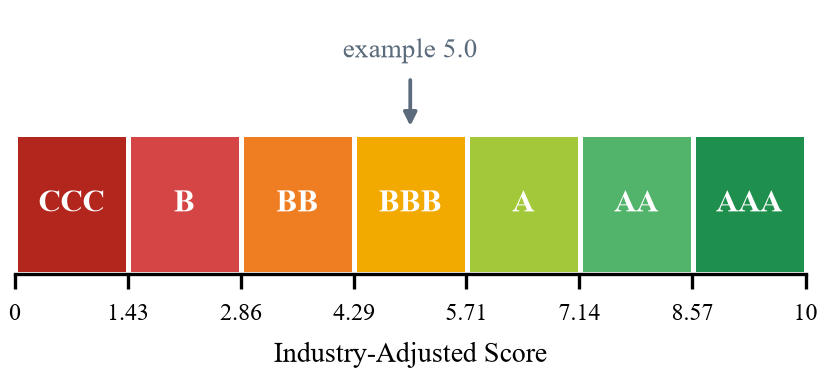
\includegraphics[width=0.95\columnwidth]{fig_v2_bands.png}
\caption{The seven rating bands on the 0-10 Industry-Adjusted Score. The marker shows an example score of 5.0 (BBB).}\end{figure}
\subsection{Differences from the MSCI Model}
Our score is MSCI-style, not an MSCI rating. MSCI measures how exposed a company is to each risk and how well it manages it, using company data, news about controversies and other sources \cite{b4}. We only have the report. A key issue score in ESGenius therefore tells how completely the report discloses what the BRSR asks for that issue. A high score means good disclosure, not good performance. Our weights are sector-level prototype values, and the industry adjustment only uses the reports analysed inside ESGenius. The application and the PDF report state this.

\section{Application Walkthrough}
This section follows one report through the application. The screens come from our test run on a public BRSR. We replaced the company name and the user e-mail on the page before taking each screenshot.

\subsection{Upload and Text Extraction}
The Documents screen (Fig. 3) is where a user starts. The user signs in, picks a company and presses Upload Document to add a PDF. Each document in the list shows its type, reporting year, upload date, size and page count, and a processing status. A new upload shows Processing while the text is extracted and changes to Ready when all pages are stored. Documents marked Shared sample belong to nobody and can only be viewed. A scanned PDF without a text layer fails at this step, because the system has no OCR. From a Ready document the user can open it with View or start an analysis with Analyze.

\begin{figure}[!t]\centering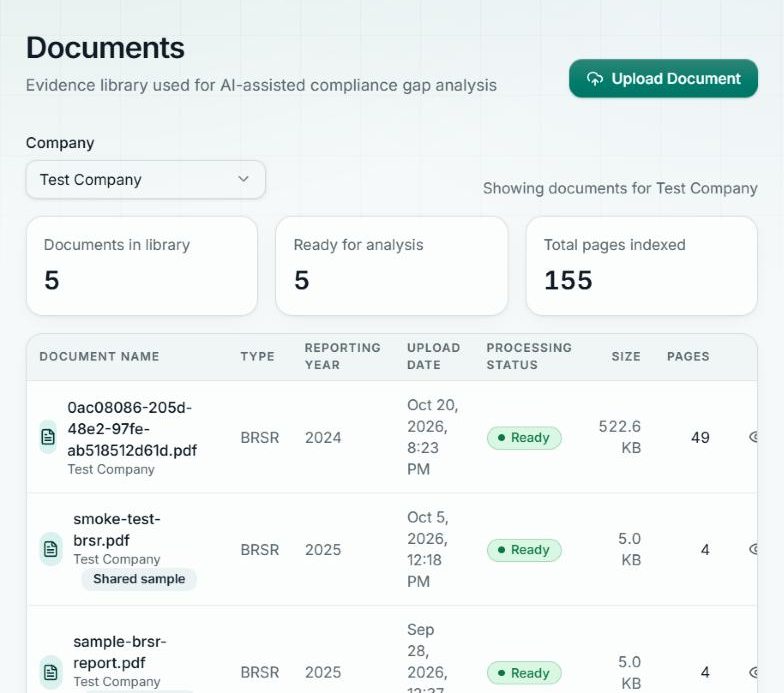
\includegraphics[width=0.95\columnwidth]{shots/documents.png}
\caption{Documents screen: the company selector, the Upload Document button and the uploaded reports with status and page count.}\end{figure}
\subsection{Running the Analysis}
After Analyze, the Compliance screen shows a progress bar with the number of requirements assessed so far and refreshes by itself. Fig. 4 shows the finished analysis of the test report. The cards at the top count the results: 41 covered, 4 partially covered, 8 not covered and 87 human review required. Below them is the list of all 140 requirements with section, indicator type, status and the confidence of the model. The list can be searched and filtered by ESG category, BRSR section, indicator type and status.

The 87 human-review items need an explanation. During this run the free daily quota of the Gemini API ran out. For 52 requirements the explanation says so, and for 35 more the classification call failed. The fail-safe rules did what they should: no requirement was guessed, and each one was handed to a person.

\begin{figure}[!t]\centering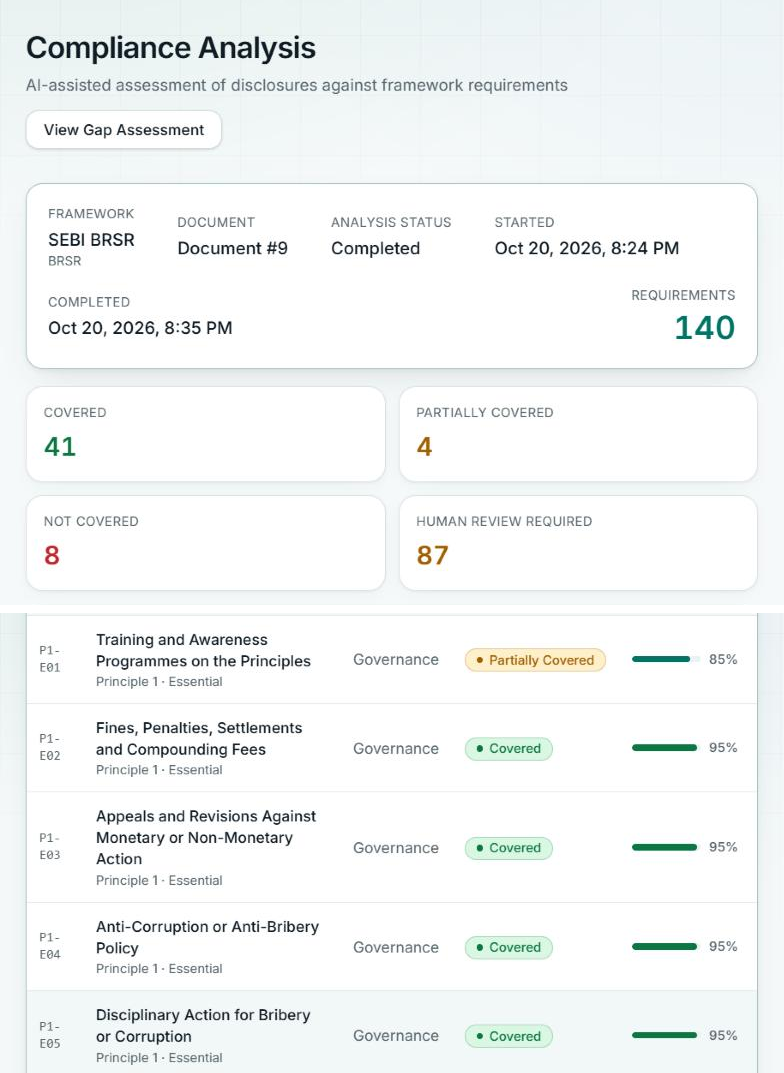
\includegraphics[width=0.95\columnwidth]{shots/results.png}
\caption{Compliance screen after the analysis of the test report: status counts and the requirement list with status and confidence.}\end{figure}
\subsection{Checking a Single Requirement}
A click on a requirement opens its detail page (Fig. 5). The page shows the status and the confidence, then the retrieved evidence with the PDF page and the retrieval score of each passage. A note says that this text comes from the document and not from the model. Under it come the explanation of the model, the identified gap and the recommendation, so the reviewer can compare the answer with the pages. The last panel is for questions that do not apply to the company. The reviewer enters a reason and presses Mark as not applicable, and the question is left out of the score from then on.

\begin{figure}[!t]\centering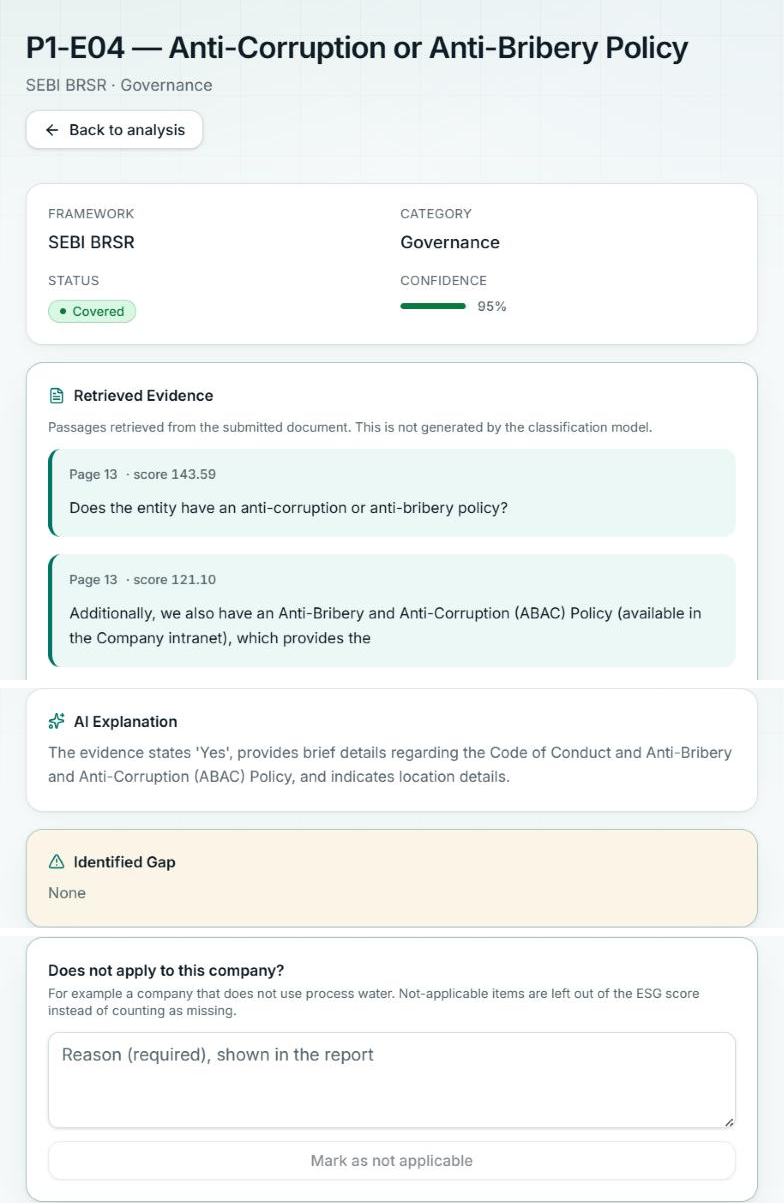
\includegraphics[width=0.95\columnwidth]{shots/detail.png}
\caption{Requirement detail: status, retrieved evidence with page numbers, model explanation, gap and the not-applicable panel.}\end{figure}
\subsection{ESG Score}
The score card sits between the status cards and the requirement list (Fig. 6). The reviewer chooses the industry from a list, here Information Technology. The card shows the rating band and the score out of 10, then the three pillar scores as coloured bars with their weights, 15\% environmental, 52\% social and 33\% governance for this industry. Below is the table of the ten key issues with their weights and scores. For this test run the weighted average is 8.2, which falls in band AA. The card says that the score is not adjusted, because only one analysis exists in this industry and at least three are needed. It also says that 53 of the 140 requirements were scored and 87 were left out while they await human review. Four key issues have no score for the same reason: all of their requirements are still waiting for a reviewer.

\begin{figure}[!t]\centering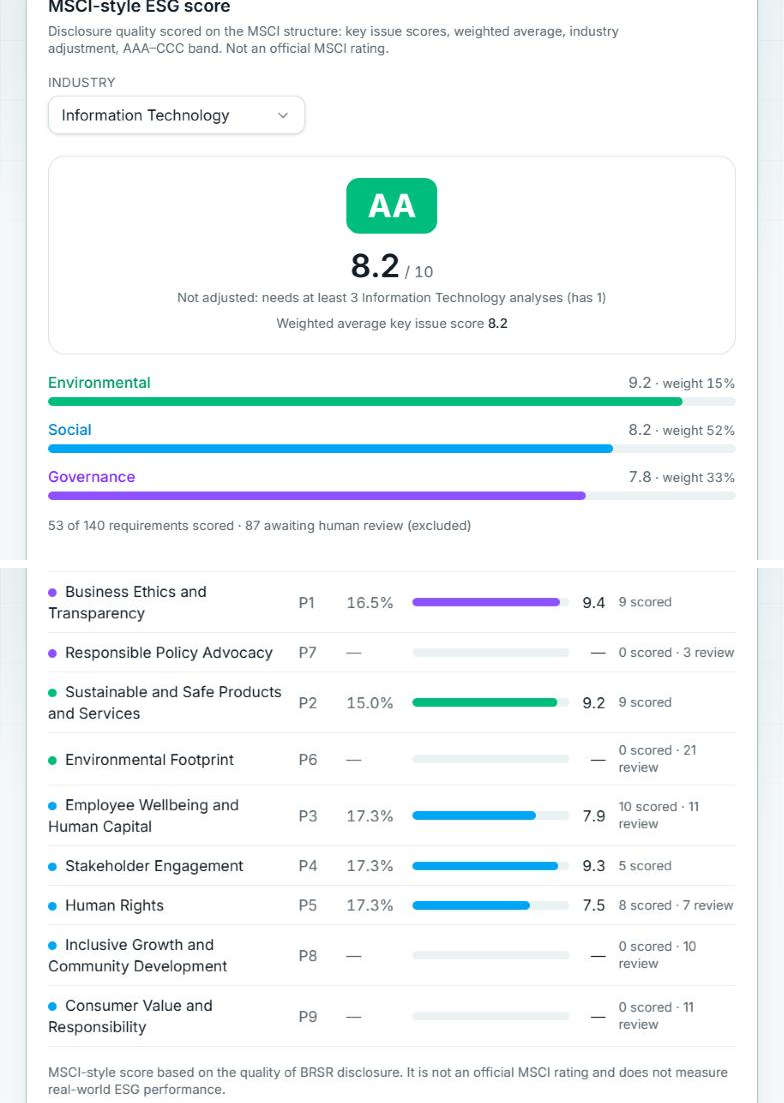
\includegraphics[width=0.95\columnwidth]{shots/score.png}
\caption{ESG score card with Information Technology selected: rating band, pillar scores with weights and the ten key issues.}\end{figure}
\subsection{Gap Assessment Report}
The View Gap Assessment button opens the report (Fig. 7). It starts with the document and analysis details and an executive summary, followed by a coverage overview with the status counts and tables by ESG category and by BRSR section. The user can print the page or download it as a PDF. The downloaded PDF also contains the ESG score, the gaps with their page citations, the human-review list and the not-applicable items with the reviewer's reasons. A disclaimer in the report says that it supports a human reviewer and is neither a certification nor an official rating.

\begin{figure}[!t]\centering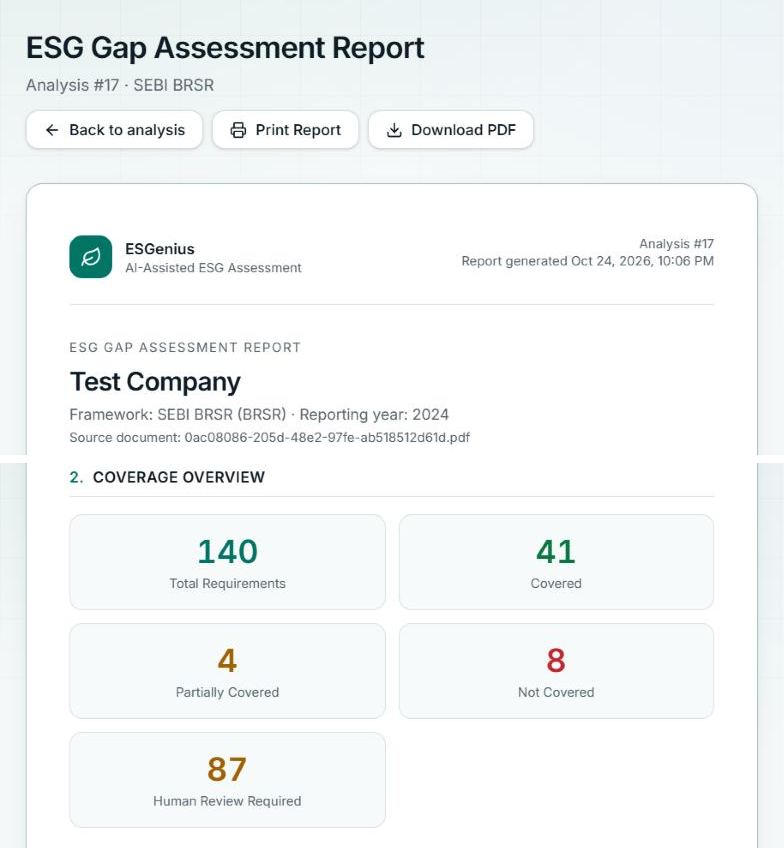
\includegraphics[width=0.95\columnwidth]{shots/report.png}
\caption{Gap assessment report screen: document details, coverage overview and the Print and Download PDF buttons.}\end{figure}
\subsection{Document Assistant}
The assistant (Fig. 8) answers a free-text question about one uploaded document. The user picks a company and a document, then types a question. The backend retrieves passages with the same search as the gap analysis and sends them to the Gemini API together with the question. In Fig. 8 the question is what evidence exists for Scope 1 emissions. The assistant quotes the sentence it found on page 34 of the test report and adds that the report gives no figures for Scope 1, which is a careful answer and not an invented number. If nothing in the document matches a question, the assistant says so and does not call the model.

\begin{figure}[!t]\centering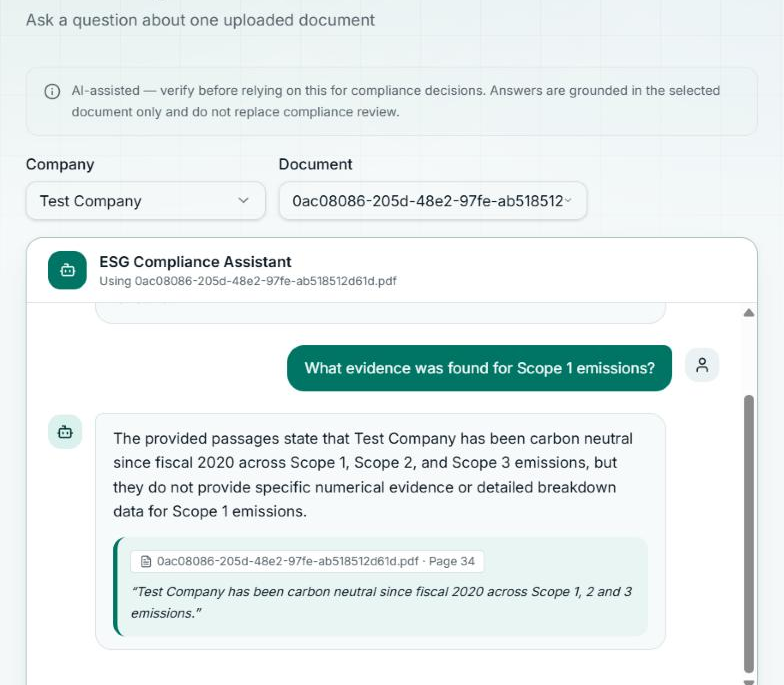
\includegraphics[width=0.95\columnwidth]{shots/assistant.png}
\caption{Document assistant: an answer to a question about the test document, with the quoted passage and its PDF page.}\end{figure}
\section{Implementation and Testing}
The backend is written in Java 21 with Spring Boot and uses a PostgreSQL database that is set up by 13 migration scripts. The frontend is written in React and TypeScript. Sign-in uses Supabase, a hosted authentication service, and a filter in the backend checks the access token on every API request.

The ESG score is calculated on request from the stored classification results. It needs no extra model calls, and it always reflects the latest industry choice and not-applicable marks of the reviewer.

The project has 393 backend tests (JUnit, one skipped) and 128 frontend tests (Vitest), 521 in total, and all of them pass. They cover retrieval, parsing of model answers, the fail-safe rules, access control, usage limits and PDF export. The scoring has 15 calculator tests, among others: full coverage gives 10, full partial coverage gives 5, weights add up to 1, not-applicable items do not change the score, and the band boundaries are right.

\section{Evaluation}
\subsection{End-to-End Run on the Test Report}
We ran a full analysis of the 49-page test report through the application. All 140 requirements were processed. 41 were classified as covered, 4 as partially covered and 8 as not covered. The other 87 became human review required, because the daily quota of the Gemini API was reached during the run (52 requirements) or a classification call failed (35 requirements). The ESG score used the 53 classified requirements. With Information Technology weights the weighted average key issue score is 8.2, and with equal pillar weights it is 8.4. Neither value is industry-adjusted, because no peer reports exist yet. Since 62\% of the requirements were not classified and the classification has not been checked against human experts, we do not read this score as a result about the company. It shows that the pipeline, the fail-safe rules and the score work together on a real document.

\subsection{Retrieval Audit on a Public BRSR}
To test the pipeline end to end we used one public BRSR of 49 pages. We do not name the company, and the report is only a test input. Retrieval ran for all 140 questions. For each question we took the highest-ranked passage and graded it as relevant, partly relevant or not relevant. An AI assistant did the grading by reading the passage and the requirement. It is a single rater and the authors have not repeated it yet, so the numbers are an estimate. Table V and Fig. 9 show the result. The retriever found evidence for all 140 questions. The top passage was relevant for 119 (85.0\%) and at least partly relevant for 129 (92.1\%). Most of the misses are short identity fields in Section A, such as addresses and contact details, and the table layout of Section B, where the nine principle columns are read line by line.

\begin{table}[!t]\centering\caption{Top-1 Retrieval Audit on the Test Report}
\footnotesize\begin{tabular}{lccccc}\toprule
Group & n & Rel. & Part. & Not & P@1 \\ \midrule
Section A & 24 & 18 & 2 & 4 & 75.0\% \\
Section B & 12 & 5 & 4 & 3 & 41.7\% \\
Principles 1-9 & 104 & 96 & 4 & 4 & 92.3\% \\
All & 140 & 119 & 10 & 11 & 85.0\% \\
\bottomrule\end{tabular}
\par\vspace{2pt}{\scriptsize\textit{P@1: share of requirements whose top passage is relevant (strict). Graded by an AI assistant.}}
\end{table}
\subsection{Behaviour of the ESG Score}
We also checked the score with the real calculator on controlled inputs. Table VI shows the WAKIS for two sectors. Full coverage gives 10 and full partial coverage gives 5 in every sector. If only the environmental sections are covered, the score is 4.5 for Energy and 1.5 for Information Technology. Energy puts 45\% of its weight on the environment and Information Technology only 15\% (Fig. 10). The last two rows show the reviewer control. When six Essential indicators of Principle 6 are not covered, the scores are 9.2 and 9.7. When the reviewer marks the same six as not applicable, both rise to 10.0, because the company no longer loses points for information it does not have. The numbers come from the same code as the application, and its unit tests reproduce them.

\begin{table}[!t]\centering\caption{Weighted Average Key Issue Score in Controlled Scenarios}
\footnotesize\begin{tabular}{lcc}\toprule
Scenario & Energy & Inf. Tech. \\ \midrule
All requirements covered & 10.0 & 10.0 \\
All partially covered & 5.0 & 5.0 \\
All not covered & 0.0 & 0.0 \\
Only environmental covered & 4.5 & 1.5 \\
Only social covered & 2.2 & 5.2 \\
Only governance covered & 3.3 & 3.3 \\
Six P6 items not covered & 9.2 & 9.7 \\
Same six marked N/A & 10.0 & 10.0 \\
\bottomrule\end{tabular}
\par\vspace{2pt}{\scriptsize\textit{Scores 0-10 from the implemented calculator; all other issues fully covered in the last two rows.}}
\end{table}
\subsection{Limitations}
We have not yet measured how often the LLM agrees with human experts. A blind study with two annotators is planned. The retrieval audit used one report and one rater. Retrieval is lexical and line-based, so multi-column tables are read less well, and scanned PDFs do not work because there is no OCR. The key issue mapping and the sector weights are our own prototype choices and not MSCI data, and the industry adjustment needs at least three reports in the same industry. The Accept AI Assessment and Mark for Human Review buttons only show a message and do not yet save a decision. Only the original BRSR format is covered, not later additions such as BRSR Core. The score measures disclosure, not performance, and every result still needs a human review.

\section{Conclusion and Future Work}
ESGenius reads a sustainability report, checks it against the 140 BRSR questions with page-cited evidence and the Gemini LLM, and turns the result into an MSCI-style ESG score with industry weights, an industry adjustment and an AAA to CCC band. Reviewers can mark questions that do not apply, and fixed rules stop the model from inventing coverage. The retrieval audit and the score scenarios show that the pipeline and the score behave as designed.

The next steps are to measure the classification accuracy with human annotators, to analyse more reports so that the industry adjustment has real peer groups, to calibrate the weights, to add table-aware retrieval and OCR, and to support more frameworks than the BRSR.

\section*{Acknowledgment}The authors thank their project mentor, Dr. Amit Aylani, for his guidance during the project.
\begin{thebibliography}{99}
\bibitem{b1} Securities and Exchange Board of India, "Business responsibility and sustainability reporting by listed entities," Circular SEBI/HO/CFD/CMD-2/P/CIR/2021/562, May 10, 2021.
\bibitem{b2} MSCI ESG Research, "ESG Ratings process," MSCI Inc., Mar. 2026. [Online]. Available: https://www.msci.com
\bibitem{b3} MSCI ESG Research, "MSCI Indicative ESG Scores methodology," MSCI Inc., Aug. 2026. [Online]. Available: https://www.msci.com
\bibitem{b4} MSCI ESG Research, "How to read your ESG rating report," MSCI Inc., 2022. [Online]. Available: https://www.msci.com
\bibitem{b5} F. Berg, J. F. Koelbel, and R. Rigobon, "Aggregate confusion: The divergence of ESG ratings," \textit{Rev. Finance}, vol. 26, no. 6, pp. 1315-1344, 2022.
\bibitem{b6} Y. Zou \textit{et al.}, "ESGReveal: An LLM-based approach for extracting structured data from ESG reports," \textit{J. Clean. Prod.}, vol. 489, Art. no. 144572, 2025, doi: 10.1016/j.jclepro.2024.144572.
\bibitem{b7} J. Ni \textit{et al.}, "ChatReport: Democratizing sustainability disclosure analysis through LLM-based tools," in \textit{Proc. EMNLP 2023 System Demonstrations}, Singapore, Dec. 2023, pp. 21-51, doi: 10.18653/v1/2023.emnlp-demo.3.
\bibitem{b8} J. A. Fernandez Fernandez, R. Kubus, and I. Martin de Santos, "Machine learning analysis of ESG score and financial health in the USA," \textit{Heliyon}, vol. 12, Art. no. e45546, 2026, doi: 10.1016/j.heliyon.2026.e45546.
\bibitem{b9} P. Lewis \textit{et al.}, "Retrieval-augmented generation for knowledge-intensive NLP tasks," in \textit{Proc. Adv. Neural Inf. Process. Syst. (NeurIPS)}, vol. 33, 2020, pp. 9459-9474.
\bibitem{b10} N. Webersinke, M. Kraus, J. A. Bingler, and M. Leippold, "ClimateBERT: A pretrained language model for climate-related text," arXiv:2110.12010, 2021.
\bibitem{b11} S. Robertson and H. Zaragoza, "The probabilistic relevance framework: BM25 and beyond," \textit{Found. Trends Inf. Retr.}, vol. 3, no. 4, pp. 333-389, 2009.
\bibitem{b12} Z. Ji \textit{et al.}, "Survey of hallucination in natural language generation," \textit{ACM Comput. Surv.}, vol. 55, no. 12, Art. no. 248, 2023.
\bibitem{b13} Gemini Team, Google, "Gemini: A family of highly capable multimodal models," arXiv:2312.11805, 2023.
\bibitem{b14} Apache Software Foundation, "Apache PDFBox." [Online]. Available: https://pdfbox.apache.org
\end{thebibliography}
\end{document}